\chapter{PCT-SCOPE-RL 与传统局部规划器的 Gazebo 公平比较}
\label{chap:pct-gazebo-benchmark}

\section{研究问题与公平性合同}
本章检验 PCT-SCOPE-RL 在修复后的 Gazebo 闭环中能否相对 Actual TEB 0.8.4 或 DWA 达到预注册
的实际性能优势。四方法共享 Autolabor M2 Ackermann 模型、$1.20\,\mathrm{m/s}$ 速度上限、
$0.60\,\mathrm{m/s^2}$ 加速、$0.90\,\mathrm{m/s^2}$ 减速、15 Hz 360 度激光、同一 warmup gate、
目标、22 s 时限和 \texttt{/cmd\_vel\_navigation} 边界。TEB 与 DWA 均在互斥开发集上评估多种
保守配置，最终采用六场景失效计入均时最强的 v0；未通过降低传统规划器性能制造优势。

主估计量为 $1-\bar T_{\mathrm{PCT}}/\bar T_b$。阳性要求点改善不少于 8\%、双侧 97.5\%
paired-block bootstrap 下界严格大于零、完成率差不低于 $-5$ pp、PCT contact 不高于基线、
mask violation 为零且统计有限。所有 timeout、未到达、负保守净空、contact 和执行完整性失败
统一以 22 s 计入。

\section{两轮独立正式研究}
R1 使用 fresh seeds 197001--197160，形成 160 个配对块、640 个 episode。PCT、解析先验、
Actual TEB 和 DWA 的有效目标分别为 153、146、89 和 80，失效计入均时分别为
15.0634、16.1231、14.9225 和 16.0881 s。PCT 相对 TEB 的降幅为 $-0.9442\%$，双侧
97.5\% 区间为 $[-8.3569\%,5.6359\%]$；相对 DWA 为 $6.3693\%$，区间
$[1.0871\%,11.1411\%]$，未达到 8\% 门。

R1 封存后仅在新开发数据中把左右低速空间候选从 0.4 改为 0.6 m/s。配对消融显示均时改善
1.2000 s，且没有降低硬安全阈值。新 pilot 按冻结功效规则选择 200 blocks，随后 R2 使用
fresh seeds 198001--198200 完成 800 个 episode。PCT、解析、TEB、DWA 的有效目标为
180、150、119、100，均时为 14.8413、16.3988、14.4470、16.0925 s。PCT 相对 TEB 为
$-2.7288\%$，97.5\% 区间 $[-9.8083\%,3.5914\%]$；相对 DWA 为 $7.7754\%$，区间
$[2.5521\%,12.6148\%]$。尽管 DWA 比较的区间下界为正，点值仍低于冻结 8\% 门，故严格
判为阴性。

\begin{figure}[htbp]
  \centering
  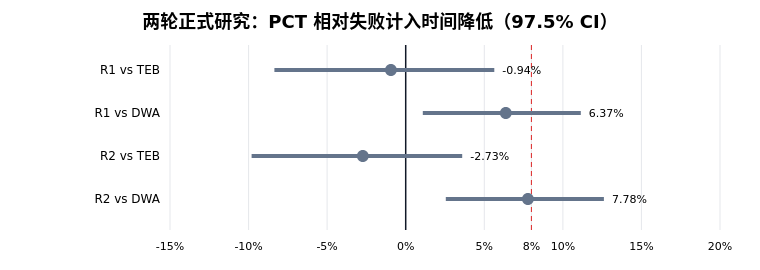
\includegraphics[width=.90\textwidth]{figures/pct_gazebo/formal_effects_97_5_ci.png}
  \caption{两轮正式研究中 PCT 相对 Actual TEB 与 DWA 的失败计入时间降幅及双侧 97.5\% 区间。}
  \label{fig:pct-gazebo-effects}
\end{figure}

\section{失败、分层与机制诊断}
R2 PCT 保留 18 次超时和 2 次保守净空失败；解析先验保留 29 次超时和 21 次 LaserScan 时间戳
TF 消息合同失败；TEB/DWA 分别保留 81/100 次负保守净空失败。PCT 相对 DWA 在部分遮挡与
静态绕障中分别快 8.3061/7.0338 s，但在 head-on 与 single-crossing 中慢 5.2666/4.6618 s。
后两层的 certified stop 和候选切换显著较多；sequential 层有 11 次 PCT timeout。这与过度停车、
切换抖动和恢复释放不足一致，但不是独立随机化因果证明。

\section{结论与边界}
两轮完整、独立、fresh-seed Gazebo 正式研究均未按预注册综合门建立 PCT-SCOPE-RL 优于 Actual
TEB 或 DWA。该阴性不推翻 V6 在冻结 fast sensor-level population 上相对解析先验的 8.4024\%
限定阳性，但阻止将其外推为 Gazebo、一般传统规划器、形式安全、部署或实车优势。未来只能在
全新 development 数据上检验安全切换滞回/停车恢复单因素，并在重新冻结和预注册后使用全新
formal seeds。
